\section{Atividade 2}

\subsection{Descrição do Modelo e Simulação}
Esta atividade envolve a criação de um diagrama de blocos no Xcos que simula a resposta de um sistema massa-mola-amortecedor com uma entrada especificada como \( f(t) = \frac{m}{5} \), onde \( m = 10 \) unidades de massa. O objetivo é analisar o comportamento do sistema sob diferentes condições iniciais e identificar métricas específicas do sistema dinâmico.

\subsection{Parâmetros do Sistema e Condições Iniciais}
Os parâmetros utilizados no modelo do sistema são:
\begin{itemize}
    \item Massa, \( m = 10 \) unidades.
    \item Coeficiente de amortecimento, \( C = 7 \) unidades.
    \item Constante da mola, \( k = 5 \) unidades.
\end{itemize}

A tabela a seguir detalha as condições iniciais ajustadas com base nos parâmetros do sistema:
\begin{center}
\begin{tabular}{|c|c|c|}
\hline
Caso & Velocidade Inicial \( V_0 \) & Posição Inicial \( X_0 \) \\
\hline
1 & \( 5 \, \text{m/s} \) (\( \frac{m}{2} \)) & \( 0 \, \text{m} \) \\
2 & \( 0 \, \text{m/s} \) & \( 2.5 \, \text{m} \) (\( \frac{m}{4} \)) \\
3 & \( 3.33 \, \text{m/s} \) (\( \frac{m}{3} \)) & \( 2 \, \text{m} \) (\( \frac{m}{5} \)) \\
\hline
\end{tabular}
\end{center}

Na verdade deixa quieto para essa atividade 1 não faz sentido o caso extra

Então vou manter os originais, te passar o tex base, as imagens geradas para sua analise e melhoria

\subsection{Resultados e Análise}
\subsubsection{Gráfico de Deslocamento}
\begin{figure}[H]
    \centering
    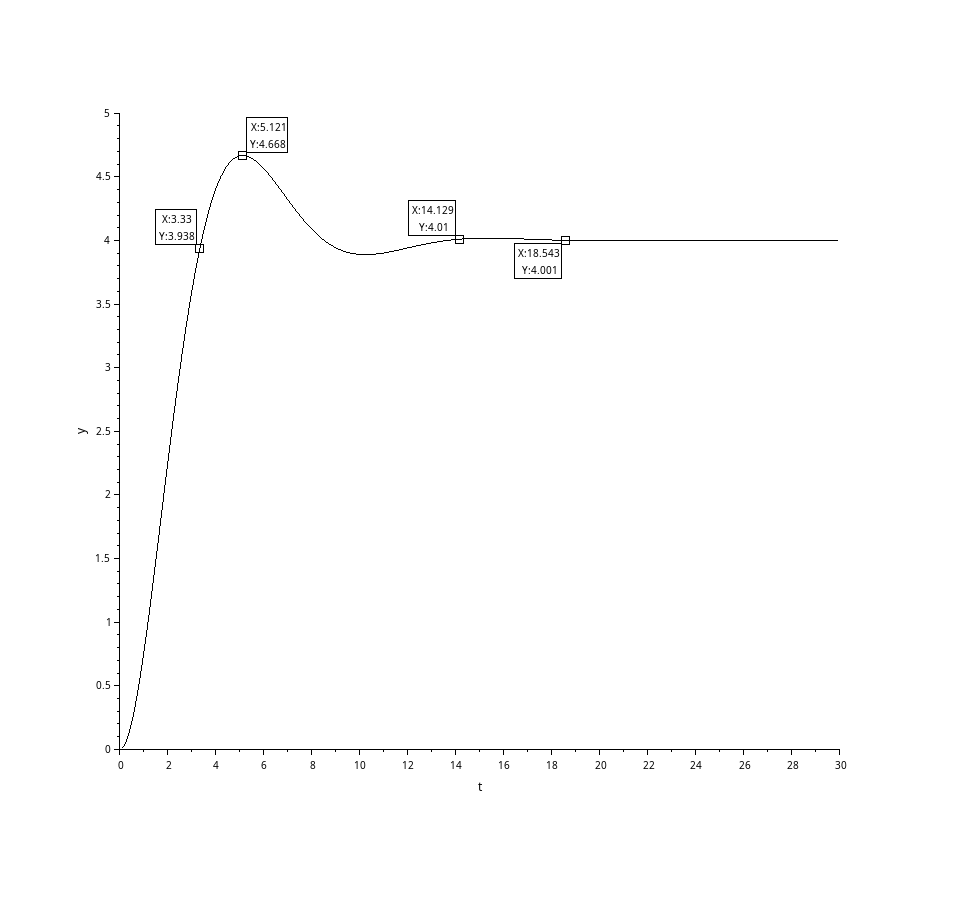
\includegraphics[width=0.7\textwidth]{2-atividade/xcos/deslocamento-caso-0.png}
    \caption{Gráfico de deslocamento com parâmetros comentados}
\end{figure}

\subsection{Resultados e Análise}
\subsubsection{Gráfico de Deslocamento}
\begin{figure}[H]
    \centering
    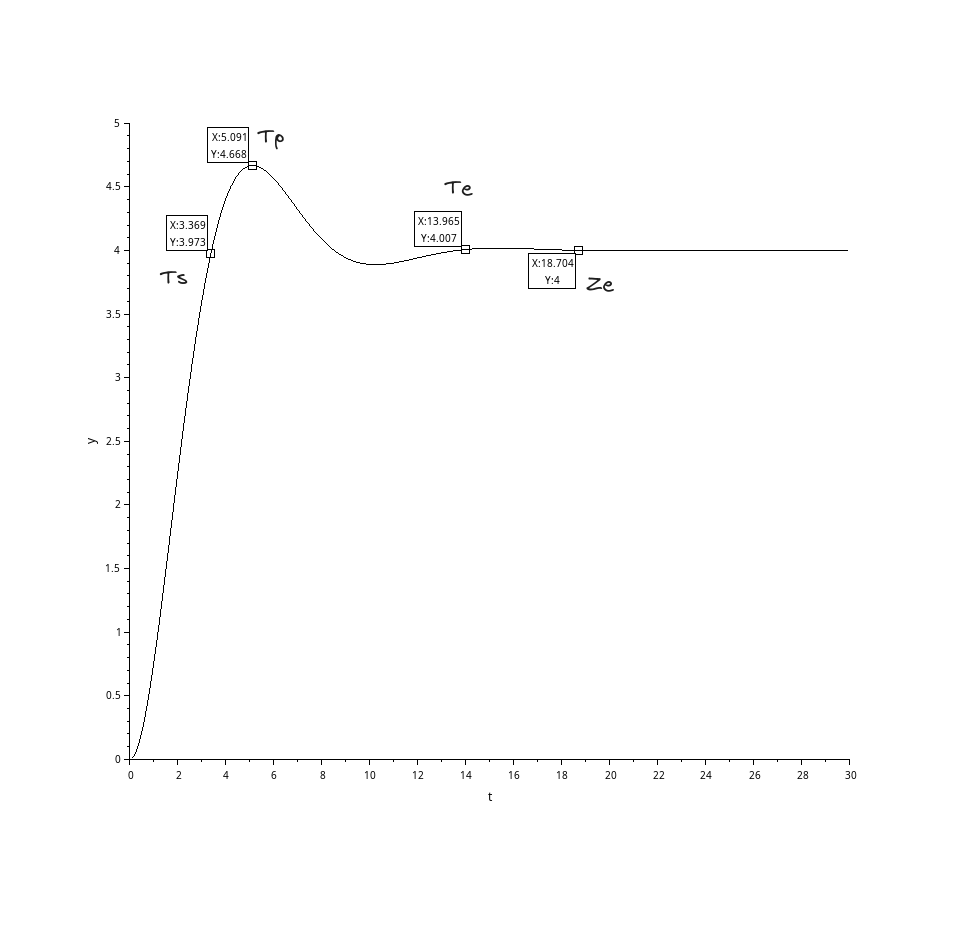
\includegraphics[width=0.7\textwidth]{2-atividade/assets/deslocamento-comentado.png}
    \caption{Gráfico de deslocamento com parâmetros comentados}
\end{figure}
No gráfico de deslocamento, são identificados os seguintes pontos:
\begin{itemize}
    \item \textbf{Tempo de Subida (Ts)}: Tempo necessário para o deslocamento alcançar pela primeira vez o seu valor máximo.
    \item \textbf{Tempo de Pico (Tp)}: Momento em que o deslocamento atinge o seu valor máximo.
    \item \textbf{Tempo de Estabelecimento (Te)}: Tempo necessário para que o deslocamento se estabilize dentro de uma faixa aceitável em torno do valor final.
    \item \textbf{Zona Estacionária (Ze)}: Região no gráfico onde o sistema mantém um comportamento constante, indicando o estado estacionário.
\end{itemize}

\subsubsection{Gráfico de Velocidade}
\begin{figure}[H]
    \centering
    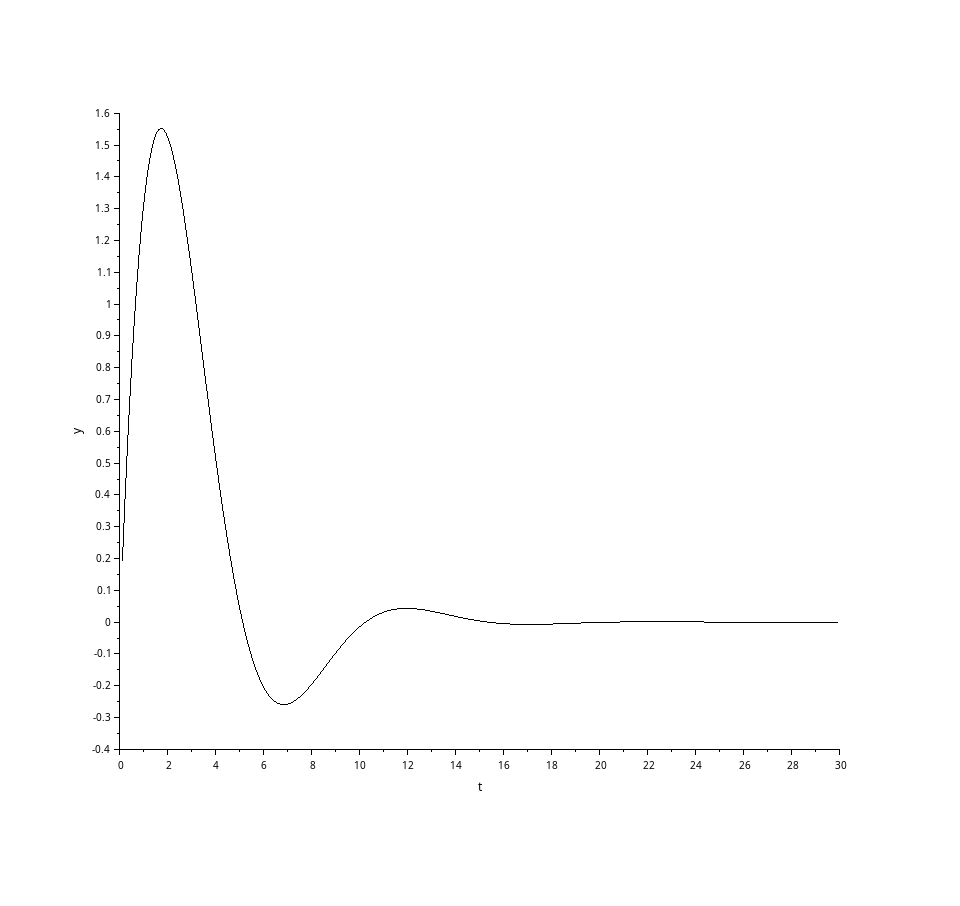
\includegraphics[width=0.7\textwidth]{2-atividade/assets/velocidade.png}
    \caption{Gráfico de velocidade}
\end{figure}
O gráfico de velocidade fornece uma visão sobre como a velocidade do sistema varia ao longo do tempo em resposta à entrada aplicada e às condições iniciais.

\subsection{Conclusões}
A análise dos gráficos de deslocamento e velocidade mostra a eficácia do amortecimento e a influência da rigidez da mola nas respostas do sistema. Cada caso demonstra um comportamento único que é crucial para entender a dinâmica do sistema sob várias condições iniciais.
